\chapter{Estruturas}
\label{chapter:estruturas}

O subsistema de estruturas, após o Ponto de Controle 2, se encarregou de fazer os ajustes finais das partes da cadeira que irão receber sensores e equipamentos eletrônicos para aquisição de sinais vitais e controle do movimento da cadeira. Para isso foi manufaturado para o último ponto de controle uma gaveta, apoio de braço e o suporte dos sensores.

Primeiramente foi realizado o sistema de gaveta que irá suportar a bateria e equipamentos eletrônicos, PCI (Placa de circuito impresso), etc. Ela foi toda elaborada de madeira adquirida no galpão da FGA, acoplada a um sistema de corrediça telescópica que está preso à estrutura da cadeira por meio de abraçadeira metálica tipo u.

Foi decidido, conjuntamente, a instalação da gaveta desta forma para assegurar a integridade da cadeira, evitando a usinagem da mesma. O sistema de corrediça foi escolhido para facilitar a remoção da bateria para recarrega da mesma, junto disso, o responsável pelo usuário da cadeira pode retirar a gaveta e conseguir fechar a cadeira para melhor mobilidade, tornando possível com que ela possa ser transportada em automóveis comuns. A Fig. \ref{fig:gaveta_aberta} mostra o sistema com a gaveta aberta, para inserção da bateria.

\begin{figure}
    \begin{center}
        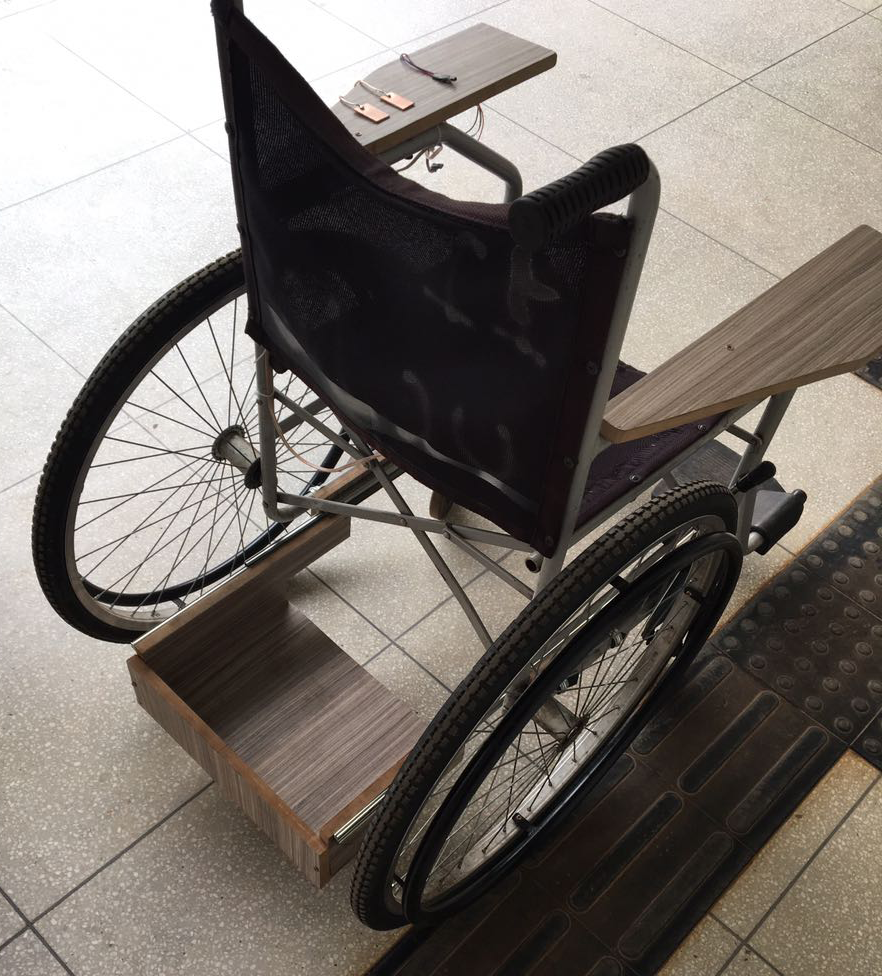
\includegraphics[width=8cm,height=8cm,keepaspectratio]{figuras/gaveta_aberta.png}
    \end{center}
    \caption{Cadeira com gaveta aberta.}
    \label{fig:gaveta_aberta}
\end{figure}

Outra manufatura foram os apoios de mão, que comportam de um lado o joystick que irá controlar os movimentos da cadeira e de outro os sensores e a \textit{Raspberry Pi}. Os apoios foram feitos de madeira (material abundante no galpão da FGA) por suas características mecânicas atenderem o projeto: resistente para a utilização e alta usinabilidade além de facilitar a inserção de equipamentos no mesmo. Os sensores foram posicionados na parte superior de um dos apoios de braço, de maneira que ao descansar o braço o usuário terá seus dados aferidos. O suporte do joystick foi medido pelo comprimento do braço de um dos membros do grupo de forma que ele seja o mais ergonômico possível e não cause desconforto ao usuário durante o funcionamento da cadeira.

Além desses sistemas,  subsistema participou  da calibragem do contato entre roda de atrito e roda da cadeira. Esta calibragem garante para os dois motores o torque aplicado a roda, assim tornando possível fazer o comando através do joystick, de forma que seja possível fazer mudanças de direção. Com estes valores fixados, diminui bastante a probabilidade de prejudicar a dirigibilidade da cadeira.

Algumas modificações podem ser feitas na cadeira de forma que o projeto atenda a maioria da população com dificuldades de locomoção e que não foram feitas por se tratar de um protótipo, falta de recursos e tempo. Por exemplo, a distância do joystick deve variar de acordo com o tamanho do antebraço do usuário, podendo ver-se para frente e para trás. Outra possível melhoria seria a inserção de um encosto removível de cabeça na cadeira, para maior conforto do paciente. Além de ter mais espaço para sensores que podem ser adicionados ao sistema caso o usuário exija maior cuidado e supervisão.

A Fig. \ref{fig:cadeira_final} mostra a estrutura finalizada da cadeira de rodas desenvolvida neste trabalho, com os suportes para todos os demais subsistemas.

\begin{figure}
    \begin{center}
        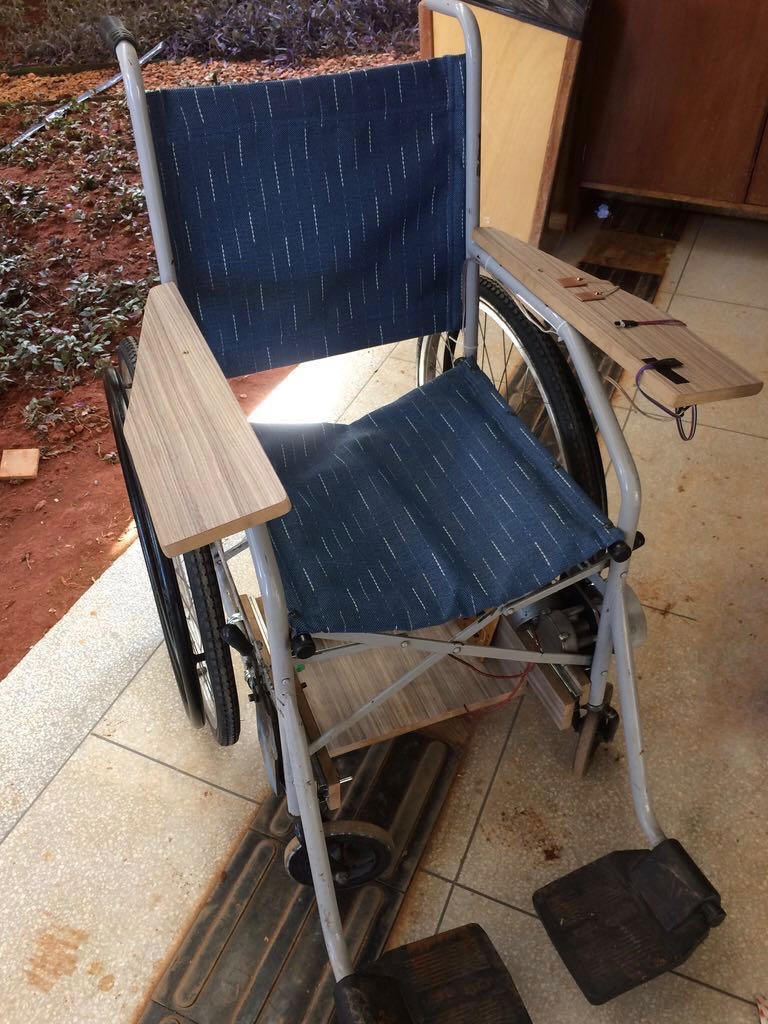
\includegraphics[width=8cm,height=8cm,keepaspectratio]{figuras/cadeira_final.jpg}
    \end{center}
    \caption{Estrutura final da cadeira.}
    \label{fig:cadeira_final}
\end{figure}
